%%
%% This is file `sample-sigconf.tex',
%% generated with the docstrip utility.
%%
%% The original source files were:
%%
%% samples.dtx  (with options: `sigconf')
%%
%% IMPORTANT NOTICE:
%%
%% For the copyright see the source file.
%%
%% Any modified versions of this file must be renamed
%% with new filenames distinct from sample-sigconf.tex.
%%
%% For distribution of the original source see the terms
%% for copying and modification in the file samples.dtx.
%%
%% This generated file may be distributed as long as the
%% original source files, as listed above, are part of the
%% same distribution. (The sources need not necessarily be
%% in the same archive or directory.)
%%
%% The first command in your LaTeX source must be the \documentclass command.
\documentclass[conference]{IEEEtran}

\usepackage[utf8]{inputenc}
\usepackage{multirow}
\usepackage[inline]{enumitem}
\usepackage{xcolor}
\usepackage{booktabs}
\usepackage{hyperref}
\usepackage{amsmath}
\usepackage{amssymb}
\usepackage{graphicx}
\usepackage[numbers]{natbib}
\usepackage{subfig}

\usepackage[nomain, toc, acronym]{glossaries}
\glsdisablehyper

\newcommand\note[2]{{\color{#1}#2}}
\newcommand\todo[1]{{\note{red}{TODO: #1}}}

%%
%% end of the preamble, start of the body of the document source.
\begin{document}

%%
%% The "title" command has an optional parameter,
%% allowing the author to define a "short title" to be used in page headers.
\title{Explainability and Adversarial Robustness for RNNs}

\author{\IEEEauthorblockN{Alexander Hartl,
Maximilian Bachl, Joachim Fabini, Tanja Zseby}
\IEEEauthorblockA{Technische Universität Wien\\
firstname.lastname@tuwien.ac.at}}

%\date{\today}

% \IEEEoverridecommandlockouts
% \IEEEpubid{\begin{minipage}[t]{\textwidth}\ \\[10pt]
%         \centering\normalsize{xxx-x-xxxx-xxxx-x/xx/\$31.00 \copyright 2018 IEEE}
% \end{minipage}}

% \renewcommand*{\bibfont}{\footnotesize}

\maketitle%

\thispagestyle{plain}
\pagestyle{plain}

\newacronym{ml}{ML}{Machine Learning}
\newacronym{dl}{DL}{Deep Learning}
\newacronym{aml}{AML}{Adversarial Machine Learning}
\newacronym{ids}{IDS}{Intrusion Detection System}
\newacronym{rnn}{RNN}{Recurrent Neural Network}
\newacronym{fgsm}{FGSM}{Fast Gradient Sign Method}
\newacronym{cw}{CW}{Carlini-Wagner method}
\newacronym{pgd}{PGD}{Projected Gradient Descent}
\newacronym{pdp}{PDP}{Partial Dependence Plot}
\newacronym{ars}{ARS}{Adversarial Robustness Score}
\newacronym{ttl}{TTL}{Time-to-Live}
\newacronym{dos}{DoS}{Denial-of-Service}
\newacronym{iat}{IAT}{Interarrival time}

\begin{abstract}

\glspl{rnn} yield attractive properties for %performing intrusion detection on network data.
constructing \glspl{ids} for network data.
With the rise of ubiquitous \gls{ml} systems, malicious actors have been catching up quickly to find new ways to exploit \gls{ml} vulnerabilities for profit. Recently developed adversarial \gls{ml} techniques focus on computer vision and their applicability to network traffic is not straightforward: Network packets expose fewer features than an image, are sequential and impose several constraints on their features. %For example, destination ports cannot be modified since that could impair communication.

We show that despite these completely different characteristics, adversarial samples can be  generated reliably for \glspl{rnn}.
To understand a classifier's potential for misclassification, we extend existing explainability techniques and propose new ones, suitable particularly % specifically crafted %AH most can also be used for non-sequential models, so lets not restrict applicability too much
for sequential data. Applying them shows that already the first packets of a communication flow are of crucial importance and are likely to be targeted by attackers. Feature importance methods show that even relatively unimportant features can be effectively abused to generate adversarial samples. We thus introduce the concept of \textit{feature sensitivity} which quantifies how much potential a feature has to cause misclassification. 

Since traditional evaluation metrics such as accuracy are not sufficient for quantifying the adversarial threat, we propose the \gls{ars} for comparing \glspl{ids} %, capturing a common notion of adversarial robustness, 
and show that an adversarial training procedure can significantly and successfully reduce the attack surface.% and improve \gls{ars}. %as a countermeasure. % AH. the score alone is not yet a countermeasure
%As a countermeasure, we develop an easy-to-use adversarial training procedure %and can confirm that it
%which significantly and successfully reduces the attack surface and improves \gls{ars}.

\end{abstract}

%%
%% The abstract is a short summary of the work to be presented in the
%% article.
%\begin{abstract}
%  A clear and well-documented \LaTeX\ document is presented as an
%  article formatted for publication by ACM in a conference proceedings
%  or journal publication. Based on the ``acmart'' document class, this
%  article presents and explains many of the common variations, as well
%  as many of the formatting elements an author may use in the
%  preparation of the documentation of their work.
%\end{abstract}

\maketitle

\section{Introduction}

There is a significant body of scientific work focusing on the detection of unwanted behavior in networks. In the past, a viable way of performing intrusion detection was to inspect the content of packets themselves and detect if a packet delivers potentially harmful content. More recently, with the increasing deployment of encryption, %available features have changed. Since payload is no longer available,
the focus now lies on features that are always available to network monitoring equipment like packet sizes, protocol flags or port numbers when encrypting above the transport layer.

Network communication is usually aggregated into \textit{flows}, which are commonly defined as a sequence of packets sharing certain properties. %, between two applications potentially being located at different physical locations.
When analyzing flows, not only the aforementioned features are available but also features related to the timing of the individual packets. % as well as their size. %AH: don't see why pkt size is not available without flows
%For example, a specific attack might require the attacker to send three small packets and the victim to reply with two large packets followed by a small one to the attacker.
Various approaches have been proposed to extract features from flows and then perform anomaly detection with the extracted flows \cite{meghdouri_analysis_2018}.
While these approaches frequently work well, it is problematic that the whole flow has to be received first and only afterwards anomaly detection is applied, revealing attack flows. Thus, we design a network \gls{ids} that operates on a per-packet basis and decides if a packet is anomalous based on features that are available even for traffic that is encrypted above the transport layer, like for example TLS or QUIC.
At the same time, an \gls{rnn}-based \gls{ids} has the benefit of providing any available information to the classifier while avoiding tedious feature engineering procedures, which derive statistical measures from the sequence of packet features.
We show that our system has similar performance to other flow-based anomaly detection systems but can detect anomalies \textit{before} the flow terminates.

However, for practical use, high detection accuracy is not enough. With the recent rise of interest in \gls{aml} techniques, also \gls{aml} for \glspl{ids} has been investigated. For example, \cite{bachl_walling_2019} investigates remedies for poisoning attacks on \glspl{ids} and \cite{hashemi_towards_2019} investigate adversarial robustness of common network \glspl{ids}.
In this research, we investigate whether adversarial samples can be found for our \gls{rnn}-based model, i.e. minimally different attack flows which are classified as benign. This is not a trivially answerable question since adversarial samples have mostly been analyzed in the context of computer vision. Our scenario significantly deviates from computer vision because \begin{enumerate*}
\item the number of features is significantly smaller and
\item only certain features can be manipulated if the flow should remain valid. % (for example the destination port cannot be manipulated)
\end{enumerate*}

Surprisingly, we can confirm that adversarial samples can be found even when considering these tight constraints. % mentioned before.
Thus, we argue that traditional performance metrics like, e.g., accuracy are not sufficient for evaluating security-sensitive \gls{ml} systems.
We propose the \acrfull{ars} as a new performance score, which captures the notion of how easily an adversary can generate adversarial samples.

Due to the threat of adversarial attacks, a further crucial requirement for \gls{ml}-based \glspl{ids} is that the classifier's decisions are interpretable by humans. This recently stirred up increased interest in explainability methods. Also in this case, common methods are designed to work with images or tabular data, but not with sequences. Hence, we extend existing explainability methods such as \glspl{pdp} \cite{friedman_greedy_2001} for sequential data. %These show the varying characteristics of different attacks and they aid with visualizing potentially vulnerable features for adversaries.
Astonishingly, feature importance methods reveal that
features, which are manipulated for successful adversarial flows,
%the that are manipulable features, that are left for modification by adversaries
are not even particularly important for the \gls{rnn}'s classification outcome. %Especially the first packets of a flow are critical for determining the decision of a recurrent \gls{ids}.
Thus, we propose \textit{feature sensitivity} methods, which show how prone a feature is to cause misclassification. 

%Since common explainability methods are designed to work with images or tabular data but not sequences, we extend existing explainability methods such as \glspl{pdp} \cite{friedman_greedy_2001} for sequential data. These show the varying characteristics of different attacks and they aid with visualizing potentially vulnerable features for adversaries.

Based on the insights gained by the feature importance and explainability methods, we propose two defense methods.
%develop a simple method for defending against adversaries who can manipulate arbitrary packets by simply leaving out potentially manipulable information from the classification process.
First, by simply leaving out manipulable features, we obtain a classifier which is slightly less accurate but is still useful to be deployed in a real scenario. Second,
by deploying an adversarial training procedure,
%AH. compared to other research about adversarial training, I dont feel that out approach is so special
%develop a custom adversarial training procedure which especially focuses on ease of use and low resource consumption and aims to keep the number of additionally introduced training hyperparameters low. With this novel strategy
we can reduce the attack surface and harden the resulting \gls{ids} while retaining all features and similar classification performance. % like for the original \gls{ml} model.

We make all the source code, data and figures freely available to enable reproducibility and encourage experimentation at \url{https://github.com/CN-TU/adversarial-recurrent-ids}.

\section{An \gls{rnn}-based Classifier}

% \begin{table}[b]
% \caption{occurrence frequency of attack types.} \label{tab:occurrence}
% \centering
% \begin{tabular}{l r} \toprule
% Attack type & Proportion \\
% \midrule
% Normal                                                         & $0.747468$ \\
% DoS / DDoS:DoS Hulk                                            & $0.101014$ \\
% PortScan:PortScan - Firewall off                               & $0.069020$ \\
% DDoS:LOIT                                                      & $0.040784$ \\
% Infiltration:Dropbox download                                  & $0.032982$ \\
% DoS / DDoS:DoS GoldenEye                                       & $0.003224$ \\
% DoS / DDoS:DoS Slowhttptest                                    & $0.001819$ \\
% DoS / DDoS:DoS slowloris                                       & $0.001680$ \\
% Brute Force:SSH-Patator                                        & $0.001107$ \\
% Botnet:ARES                                                    & $0.000327$ \\
% Web Attack:XSS                                                 & $0.000293$ \\
% PortScan:PortScan - Firewall on                                & $0.000165$ \\
% Brute Force:FTP-Patator                                        & $0.000110$ \\
% Web Attack:Sql Injection                                       & $0.000006$ \\
% DoS / DDoS:Heartbleed                                          & $0.000001$ \\
% \bottomrule
% \end{tabular}
% \label{tab:occurrence}
% \end{table}

\begin{table}[b]
\caption{Flow occurrence frequency of attack types.}
\label{tab:occurrence}
\centering
\subfloat[CIC-IDS-2017\label{fig:cicids17proportions}
]{
\begin{tabular}{l r}
\toprule
Attack type & \hspace*{-4mm}Proportion \\ \midrule
DoS Hulk	&	10.10\%	\\
PortScan, Firewall	&	6.90\%	\\
DDoS LOIT	&	4.08\%	\\
Infiltration	&	3.30\%	\\
DoS GoldenEye	&	0.32\%	\\
DoS SlowHTTPTest	&	0.18\%	\\
DoS Slowloris	&	0.17\%	\\
Brute-force SSH	&	0.11\%	\\
Botnet ARES	&	0.03\%	\\
XSS attack	&	0.03\%	\\
PortScan, no Fw.	&	0.02\%	\\
Brute-force FTP	&	0.01\%	\\
SQL injection	&	$<$0.01\%	\\
Heartbleed	&	$<$0.01\%	\\
\bottomrule
\end{tabular}
}{}
\subfloat[UNSW-NB15\label{fig:unswnb15proportions}
]{
\begin{tabular}{l r}
\toprule
Attack type & \hspace*{-4mm}Proportion \\ \midrule
Exploits	&	1.42\%	\\
Fuzzers	&	1.01\%	\\
Reconnaissance	&	0.58\%	\\
Generic	&	0.21\%	\\
DoS	&	0.19\%	\\
Shellcode	&	0.08\%	\\
Analysis	&	0.03\%	\\
Backdoors	&	0.02\%	\\
Worms	&	0.01\%	\\
\bottomrule
\end{tabular}
}{}
\end{table}

We implemented a three-layer LSTM-based classifier with 512 neurons at each layer. As the input features we use
source port, destination port, protocol identifier, packet length, \gls{iat} to the previous packet in the flow, packet direction (i.e. forward or reverse path) and all TCP flags (0 if the flow is not TCP).
% \begin{itemize*}
% \item source port
% \item destination port
% \item protocol identifier
% \item packet sizes
% \item \glspl{iat} of packets
% \item packet directions (if packet goes there or back)
% \item all TCP flags (0 if the flow is not TCP)
% \end{itemize*}.
We omitted \gls{ttl} values, as they are likely to lead to unwanted prediction behavior \cite{bachl_walling_2019}.  Among the used features, source port, destination port and protocol identifier are constant over the whole flow while the others vary.
During flow extraction we used the usual 5-tuple flow key, which distinguishes flows based on the protocol they use and their source and destination port and IP address.
We use Z-score normalization and a train/test split of 2:1.

For evaluation, we use the \textit{CIC-IDS-2017} \cite{sharafaldin_toward_2018} and \textit{UNSW-NB15} \cite{moustafa_unsw-nb15:_2015} datasets which each include more than 2 million flows of network data, containing both benign traffic and a large number of different attacks. Attacks contained in the datasets are shown in \autoref{tab:occurrence}.
\autoref{tab:performance_results} shows that our \gls{rnn}-based classifiers achieve an accuracy that is similar to previous work based on these datasets~\cite{meghdouri_analysis_2018,bachl_walling_2019}. However, unlike these classifiers, our recurrent classifier has the advantage of being able to detect attacks already before the attack flows terminate.

\begin{table}
% Evaluated using
% ./python learn.py --dataroot flows.pickle --net runs/Oct26_00-03-50_gpu/lstm_module_1284.pth --function test --batchSize 512
% ./python learn.py --dataroot flows15.pickle --net runs/Oct28_15-41-46_gpu/lstm_module_997.pth --function test --batchSize 512
% on Dec. 4th
\caption{Performance metrics per packet and per flow. MLP values from \cite{bachl_walling_2019} are presented for comparison.} \label{tab:performance_results}
\centering
\begin{tabular}{l r r r r r r} \toprule
& \multicolumn{3}{c}{CIC-IDS-2017} & \multicolumn{3}{c}{UNSW-NB15} \\
	&	Packet	&	Flow	& MLP &	Packet	&	Flow & MLP	\\	\midrule
Accuracy	&	99.1\%	&	99.7\%	&	99.8\%	&	99.5\%	&	98.3\%	&	98.9\%	\\
Precision	&	97.0\%	&	99.7\%	&	99.9\%	&	83.4\%	&	78.6\%	&	84.5\%	\\
Recall	&	97.8\%	&	99.1\%	&	99.2\%	&	87.6\%	&	72.6\%	&	82.9\%	\\
F1	&	97.4\%	&	99.4\%	&	99.5\%	&	85.5\%	&	75.5\%	&	83.7\%	\\
Youden	&	97.2\%	&	99.0\%	&	99.1\%	&	87.3\%	&	71.9\%	&	82.3\%	\\
\bottomrule
\end{tabular}
%\vspace*{-0.3cm}
\end{table}

\section{Adversarial Attacks}
\label{sec:adv}
We now investigate whether known \gls{aml} methods can be used for generating adversarial flows for our \gls{rnn}. \cite{hashemi_towards_2019} previously studied the behavior of several Network \glspl{ids} under adversarial attacks but unlike us did not investigate \glspl{rnn}.

A network packet contains significantly less features than, e.g., an image and, furthermore, most features such as TCP flags cannot be easily manipulated, as their manipulation might violate the protocol specifications and thus cause communication to fail. We identify the packet length and the \gls{iat} as features which are most likely to be exploited and thus choose them to be modified by the adversary. But even these features cannot be manipulated due to problem-specific constraints:
\begin{itemize}[topsep=0pt,wide,labelwidth=!,labelindent=0pt]
\item Only packets can be manipulated which are transmitted by the attacker, except for botnet and backdoor traffic, which is entirely controlled by an attacker and thus only packets travelling in one direction can be manipulated.
 %This means the attacker can only control one direction (except for botnets where both sides are attackers).
\item Packets must not be smaller than initially, as otherwise less information could be transmitted.
\item \glspl{iat} must not decrease, as otherwise the physical speed of data transmission can be violated in some cases. An in-depth analysis of cases in which reduction of \glspl{iat} is legitimate is complex, so we generally disallowed \gls{iat} reductions.
\end{itemize}

Several \gls{aml} methods have been proposed in the recent literature, achieving different speed-quality tradeoffs:
\cite{szegedy_intriguing_2014} shows that it is possible to create adversarial samples for an image, which look similar to the original image but are classified wrongly. \cite{goodfellow_explaining_2015} develops the \gls{fgsm}, which makes easy generation of adversarial samples possible. \cite{papernot_crafting_2016} explores the use of \gls{aml} for \glspl{rnn}, but lacks important \gls{aml} methods. %, which we consider in this paper.
% Max: But FGSM is high-speed... So I removed this paragraph altogether
%As finding adversarial flows is particularly difficult in our case, % for the reasons we discussed above,
%we preferred methods  producing high-quality adversarial samples while not being as fast as other methods.
We implemented the following \gls{aml} methods.

\subsection{Carlini-Wagner}
We implemented the \gls{cw} \cite{carlini_towards_2017}, performing gradient descent on the optimization objective
\begin{equation} \label{eq:carliniWagner}
d(X,\tilde X) + \kappa  \max(Z(\tilde X), \delta).
\end{equation}
Here, $d(\cdot)$ is a distance metric and $\kappa \in \mathbb R^+$ is a parameter governing the tradeoff achieved between attack success and distance from the original flow. Furthermore, $Z(\cdot)$ denotes the neural network's logit output, $X$ denotes the original flow and $\tilde X$ the adversarial flow optimized by \gls{cw}.

$\delta \in \mathbb R$ is a parameter that determines how far an adversary wants to exceed the decision boundary.
In the original publication $\delta=0$, meaning that the network's decision for adversarial samples is just between attack and benign traffic. In the present context, we need to make sure that the classifier's prediction would actually be benign, even though a certain level of noise will be added to \glspl{iat} due to the network between attacker and victim. Hence, we introduced $\delta=-0.2$, corresponding to a prediction confidence of 55\% for the sample to be benign after the sigmoid activation function.

We used $L_1$ as distance metric, as we consider $L_1$ distance to represent practically relevant differences of network flows best. We used \gls{pgd} for meeting the real-world constraints discussed above.

\subsection{$L_\infty$-bounded Projected Gradient Descent}
\cite{madry_towards_2018} uses a method for generating adversarial samples which deploys \gls{pgd}  to maximize the network's loss function while constraining the achieved $L_\infty$ distance from the original samples. Hence, an important difference to \gls{cw} is that for this method the network's loss instead of its logit output is considered.
We consider this method an interesting combination of \gls{cw} and \gls{fgsm}.
Since its functioning is somewhat similar to \gls{cw}, we expected the generated adversarial samples to be similarly close to the original samples.

\subsection{Fast Gradient Sign Method}
Finally, we also tested the \gls{fgsm} % which was initially proposed in
 \cite{goodfellow_explaining_2015}, which is the first method for generating adversarial samples. FGSM can be considered a single pass of \gls{pgd} on the loss function with an equality constraint on the $L_\infty$ distance, i.e. the adversarial sample is found as
\begin{equation}
\tilde X = X + \epsilon \, \text{sgn}( \nabla_X L(X)),
\end{equation}
where $L(X)$ denotes the network's loss function and $\epsilon$ denotes the achieved $L_\infty$ distance.

\begin{figure}[h]
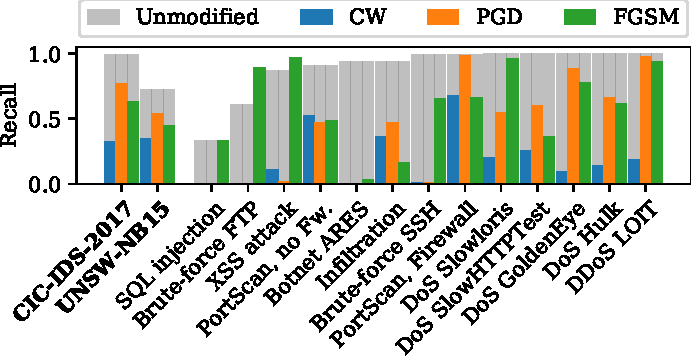
\includegraphics[width=\columnwidth]{./plots/adv_comparison/adv_comparison_17.pdf}
\caption{Attack success ratios for both datasets and per attack type for CIC-IDS-2017. Depicted are flow detection accuracies for adversarial flows and for unmodified attack flows.}
\label{fig:adv_per_family}
\end{figure}


\subsection{Evaluation}
\autoref{fig:adv_per_family} depicts the performance for the investigated algorithms for both datasets and for each attack type in CIC-IDS-2017.
We used \gls{cw} with a tradeoff of 1 and, to provide a fair comparison, for \gls{fgsm} and \gls{pgd} we used an average $L_\infty$ distance as observed for \gls{cw}.

%As expected,
\gls{cw} delivers the best performance and FGSM, while being the fastest of all investigated algorithms, delivers the worst performance.
%\autoref{fig:adv_per_family} depicts how successful the attack is for individual attack families.
The figure shows significant differences for detecting different attack families in the first place. Also for generating adversarial flows some attack families are more susceptible than others. However, the results match to a high degree with our expectations. For example, SQL injection attacks apparently are closer to benign traffic than \gls{dos} attacks and, hence, finding adversarial samples should be easier.

Interestingly, any increase of the $L_\infty$ bound for \gls{pgd} did not yield significantly improved performance. 
\gls{cw} thus generally achieved superior results to $L_\infty$-bounded \gls{pgd}
and we can confirm the recommendation by \cite{carlini_towards_2017} to perform gradient descent on the logit output instead of the loss for good results.

\autoref{fig:adv_cw} depicts the success ratio and average distance for \gls{cw} for different tradeoffs $\kappa$.
%\autoref{fig:adv_cw} depicts the ratio of attack flows which were successfully misclassified as benign with respect to the final packet along with the resulting distance from the original sample.
Evidently, the larger $\kappa$, the better the attack works, but also distances from original flows become higher. With acceptable distances, we were able to generate adversarial samples for about 80\% of attack samples.

%Note, however, that f
For successful adversarial samples, the second term in \autoref{eq:carliniWagner} becomes constant and, hence, is no longer relevant for optimization. Hence, $\kappa$ is irrelevant for the achieved distance, but governs if for one sample an adversarial sample is found.
However, when using a large $\kappa$ in \autoref{eq:carliniWagner}, to avoid overly large steps that impede convergence, it is necessary to reduce the gradient descent learning rate. Since the distance term is not affected by $\kappa$, it is furthermore necessary to scale the iteration count inversely with the learning rate. \gls{cw} with a large $\kappa$ therefore needs more time than with a small $\kappa$.


% The figure suggests that a tradeoff value between 0.5 and 1 would be ideal to find adversarial samples with a low enough distance from real samples.
% This conclusion might be misleading, however, as due to the objective function \eqref{eq:carliniWagner} the distance cannot become larger anymore for one sample as soon as an adversarial sample has been found. %, when performing optimization as depicted by the objective function .
% Hence, the depicted distance increase presumably is due to samples for which no adversarial sample could be found for lower $\kappa$ values.

\begin{figure}[t]
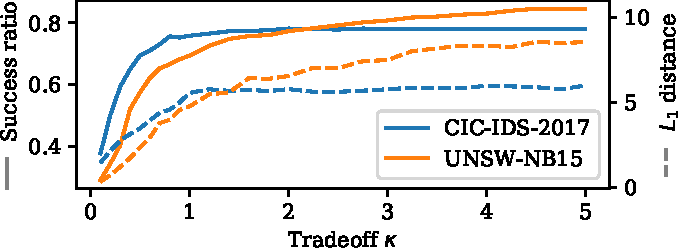
\includegraphics[width=\columnwidth]{./plots/adv_comparison/tradeoff.pdf}
\caption{Performance of \gls{cw} with different $\kappa$ values.}
\label{fig:adv_cw}
\end{figure}

\section{Evaluating Adversarial Robustness}

As \autoref{fig:adv_per_family} shows, for most attack types, most samples can be modified by an adversary to be classified as benign by using \gls{cw}. High recall for a particular attack type does not imply that adversarial samples are hard to find  %are  likely to fail
for these attacks. Thus we argue that beside the classical metrics such as accuracy, false positives etc., a metric is needed, which quantifies how easily an \gls{ids} classifier can be fooled.

Such a metric should be easy to compute and easy to interpret.
While in general adversarial robustness for \gls{ml} models is frequently quantified as the average or median of minimum distances of adversarial samples \cite{carlini_evaluating_2019}, we found no generally agreed-upon metric for \glspl{ids} in the literature. If we consider flows, for which no adversarial sample can be found, to have infinite distance, the median has the advantage of ignoring such unsuccessful samples and outliers. On the other hand, the median might depict expected distances badly if they have a very uneven distribution. 
% We propose the \gls{ars} as 
% \begin{equation}
% \text{ARS} = \text{mean}(\{d \in \mathcal D \mid d < Q_{0.5}(\mathcal D)\}),
% \text{ARS} = \frac{1}{\lceil N/2 \rceil} \sum\nolimits_{d \in \{d \in \mathcal D \mid d \leq Q_{0.5}(\mathcal D)\}} d,
% \end{equation}
% denoting by $Q_{0.5}(\cdot)$ the median, by $N = | \mathcal D | \in \mathbb N$ the total number of samples and by $\mathcal D$ the set of distances of adversarial flows from original flows, assigning unsuccessful samples a distance of $\infty$. 

We thus propose the \gls{ars} as follows. Let $\mathcal S$ denote the set of samples, $N = | \mathcal S | \in \mathbb N$ the total number of samples and $d_s \in \mathbb R_0^+$ the distance of an adversarial flow from the original flow for a sample $s\in \mathcal S$, assigning unsuccessful samples a distance of $\infty$. % and $Q_{0.5}(\cdot)$ the median function.
We define the \gls{ars} as 
\begin{equation}
\text{ARS} = \frac{1}{\lceil N/2 \rceil} \sum\nolimits_{\tilde s \in \tilde {\mathcal S}} d_{\tilde s},
\end{equation}
with $\tilde {\mathcal S} \subset \mathcal S$ denoting a set of size $|\tilde {\mathcal S}| =\lceil N/2 \rceil$, so that $d_{\tilde s} \le d_s$ for all $\tilde s \in  \tilde {\mathcal S}, s \in   {\mathcal S} \setminus \tilde {\mathcal S} $.
% We thus propose the \gls{ars} as follows. Let $\mathcal D$ denote the set of distances of adversarial flows from original flows, assigning unsuccessful samples a distance of $\infty$, $N = | \mathcal D | \in \mathbb N$ the total number of samples and $Q_{0.5}(\cdot)$ the median function.
% We define the \gls{ars} as 
% \begin{equation}
% \text{ARS} = \frac{1}{\lceil N/2 \rceil} \sum\nolimits_{d \in \tilde {\mathcal D}} d,
% \end{equation}
% with $\tilde {\mathcal D} \subset \mathcal D$ denoting the set of size $|\tilde {\mathcal D}| =\lceil N/2 \rceil$, so that for all $d \in  \tilde {\mathcal D}, d \le Q_{0.5}(\mathcal D)$.
The \gls{ars} is thus approximately the average of distances not larger than the median distance.

%Such a metric should be easy to compute, easy to interpret and robust with respect to outliers.
We consider an adversary successful if he can cause at least 50\% of all samples to be misclassified. In this case, the \gls{ars} is the average of the distances of the adversarial samples to the original samples for the 50\% of all samples which have the smallest distances. If the adversary doesn't manage to manipulate enough samples, the \gls{ars} is $\infty$.

\gls{cw} is able to find adversarial samples with minimum distance, but becomes slow for large $\kappa$. Hence, it can be used for finding the \gls{ars} efficiently as follows: 
%Since \gls{cw} becomes slow for large $\kappa$, the \gls{ars} can be efficiently found as follows:
Use \gls{cw} with a small tradeoff, trying to generate adversarial samples for an attack type. If %, of a total of $N$ samples,
 at least $N/2$  are wrongly classified, and
 the smallest distance of non-adversarial samples is not smaller than the $\lceil\frac{N}{2}\rceil$th smallest distance of adversarial samples,
stop and compute the \gls{ars}. Otherwise increase $\kappa$ and repeat. If after a predefined number of iterations -- e.g. 100 -- still not more than half of the samples are adversarial, also break and set the \gls{ars} to $\infty$.

The larger the \gls{ars} is, the more robust the model is, as then an adversary needs to modify the samples more to make them adversarial. If not more than half of the samples could be made adversarial, our metric is $\infty$ since then apparently it is not possible for an adversary to reliably conduct adversarial attacks on the majority of samples. In this case, the ratio of samples that could be made adversarial can be a useful metric to determine the exact extent of the adversarial threat.

Setting the threshold for the \gls{ars} to 50\% is arbitrary, but
 % reasonable as this way the \gls{ars} approximates the median of the distances of all samples and, additionally, marks the distance where an adversarial attack is more likely to be successful than unsuccessful.
 reasonable as outliers with very large distances are ignored and because if an attacker can make the majority of samples adversarial, we argue that its attack is ``successful''.
%we think that it is reasonable since if an attacker can make the majority of samples adversarial, we think that its attack is ``successful''.

\begin{figure}[h]
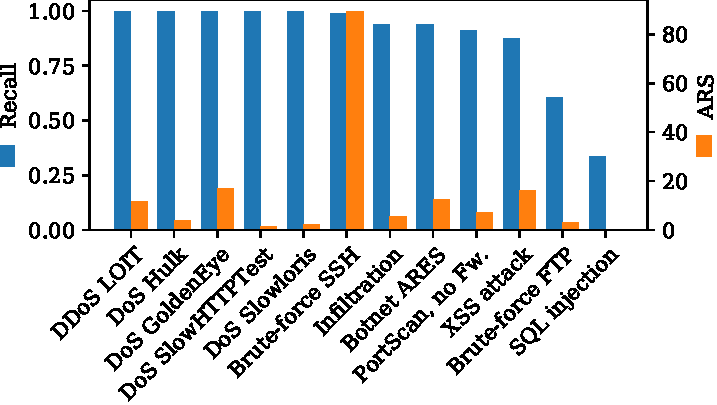
\includegraphics[width=\columnwidth]{./plots/ars_original.pdf}
\caption{Recall for unmodified flows and \gls{ars} for attacks in CIC-IDS-2017. For ``PortScan, Firewall'' recall never falls below 66\%: The attack does not succeed and the \gls{ars} is $\infty$.}
\label{fig:recall_ars}
\end{figure}

\autoref{fig:recall_ars} shows that certain attack types, like ``DoS SlowHTTPTest'', are easy to classify for an IDS but still are also surprisingly vulnerable to adversarial modifications by an attacker aiming to make them look benign.

\section{Explaining Recurrent Neural Networks}
Having verified the effectiveness of \gls{aml}  for our \glspl{rnn}, we now  investigate how the classifiers come to a decision.
From a naive perspective, one might be tempted to reuse existing explainability methods for \glspl{rnn} by considering a flow the sum of its packet features.
We identify several difficulties which occur when trying to explain decisions made by \glspl{rnn}.

\begin{itemize}[topsep=0pt,wide,labelwidth=!,labelindent=0pt]
\item
\textbf{Feature quantity.}
The number of features fed into an \gls{rnn} is the number of packet features times the length of the flow. For long flows, the total number of inputs can become very large.

\item
\textbf{Variable sequence lengths.}
The length of different flows might differ tremendously. Hence, features at one particular time step might be important for the network's outcome for one flow, but not even exist for other flows. 

\item
\textbf{Lack of a distance measure.}
However, even if we restricted the analysis to flows of a constant length, a flow is different from the plain concatenation of its packet features.
For example, in a sentence, which is sequence of words, parts can be rearranged, giving a different sequence with possibly the exact same meaning. 

\item
\textbf{Multiple prediction outputs.}
Often an \gls{rnn} produces an output at each time step. When  applying explainability methods, the question arises which output to consider for the method. The natural choice is to base the methods on the prediction output which occurs at the same time step as the feature under investigation: This approach is less complex compared to considering also features of all earlier time steps. Also, we expect the current prediction outcome to more dependent on the current feature, compared to a feature from many steps ago. 
However, due to the complex decision processes of deep neural networks,
this is not always true and a feature might influence a decision many time steps later. 
\end{itemize}

Many explainability methods proposed recently are local and thus provide explanations for a particular data sample \cite{shapley_value_1953,lundberg_unified_2017,dhurandhar_model_2018,ribeiro_why_2016}. However, for the particular problem of network traffic, due to the high number of flows and the characteristics of data, analyzing individual samples is of low interest. Explainability methods presented in this paper therefore aim to understand a model by analyzing which features are important, at which time step they are important and which feature values lead to classification as attack.

% where does this come from :)
%\subfloat[Throughput of the fq \gls{qdisc}\label{fig:fqThroughput}
%]{
%\includegraphics[width=\columnwidth]{{{plots/throughput_1_fq_cubic_10_20_60_0.5_bw_1571240937211.pcap}}}
%}{}

\subsection{Feature Importance Metrics}
%\begin{table}
%\caption{Accuracy drop for:}
%\label{tab:feat_importance}
%\centering
%\subfloat[Random replacement method\label{fig:featRandom}
%]{
%\begin{tabular}{l r}
%\toprule
%Feature & \hspace*{-4mm}Accuracy~drop \\ \midrule
%Protocol & 0.207 \\
%Packet Length & 0.165 \\
%SYN Flag & 0.099 \\
%ACK Flag & 0.084 \\
%Direction & 0.073 \\
%Destination port & 0.071 \\
%Source port & 0.060 \\
%RST Flag & 0.057 \\
%PSH Flag & 0.056 \\
%Interarrival time & 0.024 \\
%FIN Flag & 0.012 \\
%URG Flag & 0 \\
%ECE Flag & 0 \\
%CWR Flag & 0 \\
%NS Flag & 0 \\
%\bottomrule
%\end{tabular}
%}{}
%\subfloat[Feature dropout\label{fig:featDropout}
%]{
%\begin{tabular}{l r}
%\toprule
%Feature & \hspace*{-4mm}Accuracy~drop \\ \midrule
%Destination port & 0.025 \\
%Source port & 0.003 \\
%RST Flag & 0.001 \\
%ACK Flag & 0.001 \\
%Protocol & 0.001 \\
%Packet Length & 0.001 \\
%Direction & 0.001 \\
%SYN Flag & 0 \\
%Interarrival time & 0 \\
%FIN Flag & 0 \\
%ECE Flag & 0 \\
%URG Flag & 0 \\
%CWR Flag & 0 \\
%NS Flag & 0 \\
%PSH Flag & 0 \\
%\bottomrule
%\end{tabular}
%}{}
%\end{table}
As a first step to understanding the neural network's decisions, we  estimate how important individual features are for the model's predictions.
When investigating an \gls{ml} classifier, it is natural to ask which inputs have a large influence on the classifier's prediction. We feel the need to distinguish metrics for this purpose based on their main aim:

A large amount of research has been spent on finding \emph{feature importance} metrics, which allow the selection  of high-importance features, providing a reasonably good classification performance while resulting in a more light-weight classifier.

Conversely, both adversarial machine learning and explainable machine learning bring up the question to what extent individual features are able to change the prediction outcome. While appearing similar, traditional feature importance can yield markedly wrong results for this case.  To distinguish, we propose the term \emph{feature sensitivity} for such metrics.
To analyze features, we use the following approaches:

\subsubsection{Neural Network Weights}
In previous works~\cite{olden_accurate_2004}, a simple method for determining feature importance in neural networks has been summing up neural network weights leading from a certain input to the prediction outcome. The weights method can be considered for both feature importance and feature sensitivity, however, clearly, especially in the case of complex network architectures, this method is likely to provide wrong results. Hence, we provide results for the weights method mainly for comparison. Note that an LSTM cell alone has four weights leading from one input to an output.

\subsubsection{Input Perturbation}

The most commonly deployed feature importance techniques, used by practitioners for \glspl{rnn} \cite{stackexchange_cross_validated_neural_2019} and \gls{dl} \cite{molnar_interpretable_2019,stackexchange_cross_validated_feature_2016,olden_accurate_2004}, are based on adding noise to a particular feature and evaluating the drop in accuracy that occurs. We argue that it is hard to determine the ``correct'' intensity of noise to add. %, we slightly vary the proposed approach: We do not add noise drawn from a probability distribution but instead
 Hence, we sample the value for a feature from the distribution of all values of this feature in the dataset. This makes the method non-parametric since the noise distribution  does not need to be chosen. We ensured that features which stay constant for a flow, i.e. source port, destination port and protocol, also stay constant throughout the flow when randomizing the feature.


\subsubsection{Feature Dropout}
While the perturbation method %of adding noise to features/randomizing them
is convenient since it is easy to implement and understand, we argue that it has some shortcomings:
The \gls{rnn} was never trained for dealing with ``garbage'' values that the randomization creates. For example, completely unrealistic feature combinations could occur that were never observed during training. Furthermore, sequences of features could occur that cannot occur in reality.

%We think that the ``ideal'' feature importance method for our scenario are Shapley values \cite{shapley_value_1953}: To analyze feature importance with them, the feature under investigation is completely omitted from the dataset and a model is trained without it. The resulting accuracy is then compared to the baseline accuracy with all features. The effort required to do this is high both in terms of storage space as well as training time since for $n$ features $n$ models need to be separately trained and stored. While this seems tractable, when also analyzing the feature importance of combinations of features, the number of models required becomes even larger: Out of $n$ features, $2^n$ unique subsets can be chosen, meaning that the computational demand rises exponentially.

To evaluate true feature importance, we thus develop a more sound method %compared to input perturbation
called \textit{feature dropout}: When training a model, for each sample, we leave out each feature  with independent probability $\frac{1}{n}$, $n \in \mathbb N$ being the number of features, by setting it to zero. On average, one feature gets zeroed out but it is also possible that none or more than one are left out. This procedure is equivalent to using dropout \cite{srivastava_dropout:_2014} with probability $\frac{1}{n}$ before the first layer.

An important implementation detail is that for each feature we add another input which is 1 if the feature is suppressed and 0 otherwise. This is necessary for the neural network to be able to distinguish between a feature missing and a feature genuinely being zero. The overall outcome is a classifier being able to deal with missing features.
The results in \autoref{fig:feat_imp} show that, unlike input perturbation, feature dropout  does not vastly overestimate features' importance. With feature dropout, it becomes apparent that only very few features  actually contain unique information, affecting accuracy when left out: the destination port and the source port.

A model trained with feature dropout typically yields slightly lower accuracy than a regularly trained model, even if no features are left out (flow accuracy of 99.43\% vs. 99.65\%). We thus recommend training two models: One regular one and one with feature dropout to use for the feature importance.

Another method that uses dropout for feature importance is \cite{chang_dropout_2017}, applying a technique called \textit{Variational Dropout} to learn the optimal dropout rate for each feature. It tries to leave out as many features as possible and at the same time keep accuracy high. Thus important features are going to be left out less often and one can then extract the dropout probabilities for each feature and assess their significance based on them. %
% Max: I'd say that the following sentence is optional...
While this method looks seemingly related to feature dropout, it is significantly more complex and does not aim to show the accuracy drop that occurs when omitting a feature but instead returns a unique feature importance value between 0 and 1. 
%Feature dropout can also be used as a building block for computing the accuracy of datapoints with missing features that is necessary to compute Shapley values \cite{shapley_value_1953} or KernelSHAP \cite{lundberg_unified_2017}.

For feature dropout, it can also happen that several features are left out for a sample and so our method can also be used to analyze the effect of multiple features missing and can thus show possibly correlated features or -- more general -- features that contain common information, relevant for the classification task:
%Feature dropout also allows us to find correlated features or -- more general -- features that contain common information:
\begin{equation}
\text{score} = \frac{\text{acc}_{\text{base}}-\text{acc}_{\text{-both\_features}}}{\left(\text{acc}_{\text{base}}-\text{acc}_{\text{-feature\_1}}\right) + \left(\text{acc}_{\text{base}}-\text{acc}_{\text{-feature\_2}}\right)}
\end{equation}
With $\text{acc}_{\text{base}}$ we denote the accuracy of the classifier with all features included, with $\text{acc}_{\text{-feature\_i}}$ the accuracy if feature $i$ is omitted and with $\text{acc}_{\text{-both\_features}}$ the accuracy if both features are omitted. Assuming a non-negative accuracy drop when omitting a feature, the resulting score is $\ge 0.5$. The higher it is, the larger the information that both features share.

%AH. As it can become <1, I would say it this way
%If the score is one,  both features contain no joint information.
For example, the score between RST and the protocol identifier is 8.5; the highest of all pairs of features. While this may be unintuitive at the first glance, it likely stems from the fact that if the protocol identifier (TCP or UDP) is missing, then 
%if RST is 1 at some point of a flow, it has to be TCP.
RST being 1 at some point indicates that the flow is TCP.

Feature dropout might constitute a building block for methods based on Shapley values \cite{shapley_value_1953} like KernelSHAP \cite{lundberg_unified_2017}. 
%Due to space limitations, we leave this for future work.
\subsubsection{Mutual Information}
\begin{figure}
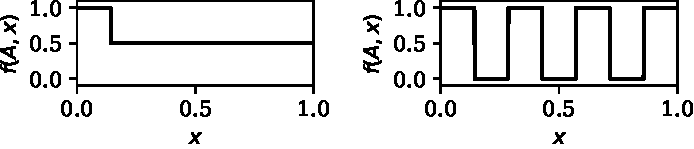
\includegraphics[width=\columnwidth]{./plots/mutinfo_example.pdf}
\caption{Two distributions yielding an identical accuracy drop.}
\label{fig:mutinfo_example}
\end{figure}
Input perturbation and feature dropout mainly address feature importance.
For example, assuming that the test dataset is representative for production use, for feature importance it is reasonable to equate the distribution for perturbing a feature with the feature distribution itself. However, when evaluating feature sensitivity, e.g. for analyzing potential for adversarial samples, the attacker is not limited by this distribution and frequently is able to choose arbitrary values in the feature space.

\begin{figure*}
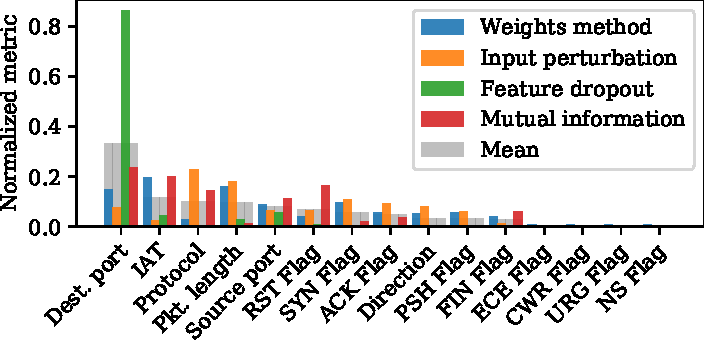
\includegraphics[width=.49\textwidth]{./plots/importance/feat_imp_flow_2017.pdf}\hspace{.02\textwidth}
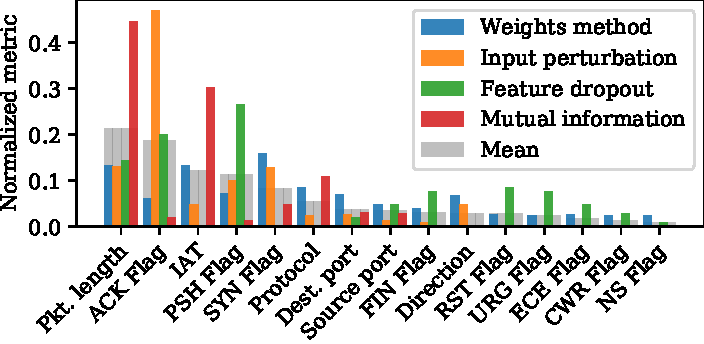
\includegraphics[width=.49\textwidth]{./plots/importance/feat_imp_flow_2015.pdf}
\caption{Feature importance metrics for the flow prediction for CIC-IDS-2017 (left side) and UNSW-NB15 (right side).}
\label{fig:feat_imp}
\end{figure*}
Furthermore, let $f(A,x)$  denote the joint probability
%\todo{Max: Ist joint probability nicht immer wenn man mehrere Ereignisse hat? Ich hätte hier probability density function geschrieben...}
%AH. changed notation and wording
for classification as attack and a feature value $x$. Accuracy then is $\int f(A,x) dx$ for attacks and $1-\int f(A,x) dx$ for benign traffic.
\autoref{fig:mutinfo_example} shows two different distributions
yielding the same accuracy, but clearly the right-side distribution has a larger influence on the prediction, as in the right-side case the prediction deterministically depends on the feature value.
To capture such dependencies, we propose to use mutual information %instead of accuracy drop
to determine feature sensitivity.
Mutual Information between two random variables $X,Y$ is defined as
\begin{equation}
I_{X,Y} = \mathbb E \left\{ \log\left(\frac{f_{X,Y}(x,y)}{f_X(x)f_Y(y)}\right) \right\},
\end{equation}
with $f_X(x), f_Y(y)$ and $f_{X,Y}(x,y)$ denoting the distribution of $X,Y$ and their joint distribution, respectively. To obtain feature sensitivity, we compute mutual information between an input variable and the prediction output for one flow at one particular time step, averaging over the result for the test set.

\subsubsection{Comparison}
\autoref{fig:feat_imp} shows the results, which match to a large extent with domain-specific expectations for classifying network flows.
In particular, rarely used TCP flags like NS or URG are unimportant for the classifier. On the other hand, destination port and protocol are essential for characterizing flows by hinting at the type of traffic. \gls{iat} and packet length are important for estimating the amount of transferred information and several flags hint at certain attacks like \gls{dos} attacks.

The weights method is able to reveal features with a very low importance to a certain degree, but disagrees with the other methods to a large extent. Less anticipated, however, also input perturbation does not exhibit a considerable correlation with feature dropout. Considering its functioning of completely removing individual features, feature dropout is the most reliable method for evaluating importance for removing features. It is remarkable that none of the other methods is able to depict the distinct peak of importance for the destination port.

It is not surprising that mutual information disagrees with feature dropout, since both their aim and their functioning are substantially different. For example, mutual information shows that the protocol field can have a substantial impact on the classification even though an identical accuracy can be achieved when omitting it.

% In particular, the most important features turn out to be the used protocol, packet length and the SYN TCP flag. While the first two features are essential for characterizing flows, a high number of packets with set SYN flag is an important characteristic for port scanning or certain DoS attacks. Also the fact that most of TCP flags do not play an important role in our dataset was expected. It is interesting to note, however, that the interarrival time of packets does not play a crucial role for the detection of attacks.

Metrics for UNSW-NB15 differ substantially from CIC-IDS-2017. However, due to the large number of different network attacks and network configurations, it is easily possible that relevant features are very different. We consider the question of model transferability of substantial importance for \gls{ids} applications, but out of scope for the present research.

\subsection{Explainability Plots}
Knowing which features to investigate, it is important to analyze which feature values lead to classification as attack.
In literature, the use of Partial Dependency Plots (\gls{pdp}) has been proposed~\cite{friedman_greedy_2001}. To inspect attack types in detail, in this research we use a \textit{conditional} form of the \gls{pdp}. If $\boldsymbol X \in \mathbb R ^n$ denotes a random vector drawn from feature space, $f(\boldsymbol X) \in [0,1]$ the neural network's prediction and $c$ the attack type, we define the conditional \gls{pdp} for feature $i$  as
% \begin{equation} \label{eq:pdp}
% \text{\gls{pdp}}_i(y) = \mathbb E_{\boldsymbol X}\left(f(X_1,\ldots,X_{i-1},y,X_{i+1},\ldots X_n)\right)
% \end{equation}
% To inspect attack types in detail, in this research we experiment with a modified definition of the \gls{pdp}  (with C being the attack classes):
\begin{equation} \label{eq:pdp_conditional}
\text{\gls{pdp}}_{c,i}(w) = \mathbb E_{\boldsymbol X | C} \Big(f \left( X_1,\ldots,X_{i-1},w,X_{i+1},\ldots X_n \right) | c\Big),
\end{equation}
empirically approximating the conditional distribution by the observed subset that belongs to a certain attack type.

By using a classical \gls{pdp} we would likely lose information due to the averaging over very different types of traffic. However, for network traffic in particular, investigating each sample individually is not possible. Hence, the conditional \gls{pdp} provides the ideal compromise for our application.

Due to the use of a 5-tuple flow key, port numbers and the protocol identifier are constant for all packets in one flow.
Hence, we can consider the \gls{rnn} a regular classifier and reuse 
%which allows us to use
\glspl{pdp}, which have been proposed for non-recurrent classification methods, by plotting the \gls{rnn}'s flow prediction outcome over one of these  features.
The results (omitted for brevity) show that for some attack types the port numbers play an important role. When looking at the \gls{pdp} for benign traffic samples, %(non-attack traffic)
it becomes apparent that traffic destined to a high destination port is generally indicative of an attack. We argue that this is because most services that regular users use have low port numbers.

\subsection{Plots for Sequences}

%As apparent from the above discussion, trying to explain how packet features influence the model's predictions, poses various difficulties. As a first step to explaining our model's predictions, we investigate how important features at different time steps are for the model's decisions.
Intuitively, features at the beginning of a flow should be the most important while the classifier's predictions should not vary significantly anymore, as soon as it has come to a decision.
\begin{figure}
\includegraphics[width=\columnwidth]{{"./plots/plot/flows_pred_plots2_outcomes_0_3.pickle_15_All_samples"}.pdf}
\caption{Classifier confidence per time step for CIC-IDS-2017. % and first and third quartiles.
For the majority of attack types, confidence increases in the first few steps and then stays almost constant at 1.}
\label{fig:confidence}
\end{figure}
To evaluate this hypothesis, \autoref{fig:confidence} depicts the classifier's prediction confidence for each time step, along with the number of samples having at least this length, which were used for evaluating the figure. % for each attack class.
%averaging over all flows. %AH. there's no averaging happening
% and also show the first and third quartiles.
%\autoref{fig:confidence} shows that %this hypothesis is correct for most attack classes.
While at the first couple of packets the confidence is not very high, towards the end of the flow it reaches values close to 1 and stays there. Hence, not only is the classifier able to make a reasonable classification after just a few packets, the figure also suggests that indeed later packets have a neglectable influence on the prediction.

For investigating in more detail how features influence the prediction outcome, we extend \glspl{pdp} to the sequential setting.
Denoting as $X=\{\boldsymbol X^1, \ldots, \boldsymbol X^m\}$ the series of packet features $\boldsymbol X^t \in \mathbb R^n$ and $h_t(X)$ the network's hidden state after time step $t$, we define the sequential \gls{pdp} as
\begin{align}
\text{se}&\text{qPDP}_{c,i}(t,w)= \\ &\mathbb E_{X | C} \Big(f \left(h_{t-1}( X), X_1^t,\ldots,X_{i-1}^t,w,X_{i+1}^t,\ldots X_n^t \right) | c\Big). \nonumber
\end{align}

\autoref{fig:pred_plots2} shows an example together with the mean values for both unmodified samples and adversarial samples. Also in this figure we notice that mainly the first few packets are able to influence the prediction outcome and modifying features at a later time step does not change its confidence any longer. In many cases, the adversarial sample generation indeed moves packet features to areas where the network is less likely to be classified as attacks, confirming the effectiveness of \glspl{pdp}. In other cases, however, we did not observe an agreement between \gls{pdp} and adversarial modifications, hinting at dependencies which cannot be presented by \glspl{pdp}. Since the \gls{iat} is undefined for the first packet, we always set it to 0. Still, interestingly, the plot shows, that the classifier considers packets with a higher IAT to be more likely to be attacks than those with a smaller one. 

\begin{figure}[h]

\includegraphics[width=\columnwidth]{{"./plots/plot2_adv/flows_pred_plots2_outcomes_flows_adv_1.0_notBidirectional_outcomes_0_3.pickle_0_3.pickle_7_DoS_-_DDoS-DoS_slowloris"}.pdf}

\caption{Exemplary sequential PD plot and adversarial flows for the DoS Slowloris attack in CIC-IDS-2017. The lines show the feature's mean values. % for all flows of the attack type.
The shaded region shows the change in confidence that occurs when the feature is varied.}
%\todo{IAT plot is wrong: There shouldn't be step 0.} %AH. guess this is fine now
\label{fig:pred_plots2}
\end{figure}

% AH. I guess this can only be properly formulated with a formula
%Next, we want to investigate if our classifier just memorized its inputs. The most interesting packet features that can be used to visualize this in our use case are the \gls{iat} between packets in a flows and the packet length. To depict how the model comes to a decision, we determined the total minimum and maximum for these features that ever occur for all flows. For a given flow $X$ we then varied feature values at each time step between minimum and maximum and plot how the confidence changes when the feature varies (\autoref{fig:pred_plots2}) depict the averaged predictions for different attack families.

%Furthermore, it seems clear that the classifier did not just memorize the inputs but actually learned appropriate space representations, as there is always a smooth decrease of confidence when modifying feature values. When memorizing, we would  instead expect a sharp decline of confidence. 
% to occur.
%Another interesting observation is that after the first couple of packets the classifier is certain about its decision and changing features doesn't change its confidence any longer. This allows the conclusion that if an attacker is able to change the first few packets, she could change the decision of the classifier. This is consistent with our observations in \autoref{sec:adv}. %We will further investigate this question in \autoref{sec:adv}.

\begin{figure}
%AH. I think the 'Firewall off' plot is not a good example as it shows only 4 packets
\includegraphics[width=\columnwidth]{{"./plots/plot_features/flows_pred_plots2_outcomes_0_3.pickle_2_Brute_Force-SSH-Patator"}.pdf}
\caption{\gls{iat} and packet length for SSH brute-force attacks in CIC-IDS-2017.}% The solid line shows the median value of the feature for all flows of a specific attack type. The shaded region are the first and third quartile.} % think legend is enough for unterstanding
\label{fig:plot_features}
\end{figure}
Finally, we investigated whether our classification task involves recognizing complex patterns in the feature space.
As example, \autoref{fig:plot_features} shows that
%Looking at the plots of the features that vary over time (\autoref{fig:plot_features}) we see that certain
attack types indeed have a characteristic pattern in which they send packets by which they are easily recognizable.
Other attack families similarly show characteristic patterns.
%We want to determine how the pattern of packet sizes and \glspl{iat} is significant for the classification. \autoref{fig:plot_features} clearly shows that some attack types have very characteristic patterns of packet sizes and \glspl{iat}.

\section{Defenses}
We now investigate two approaches to increase robustness of the \glspl{rnn} against adversarial attacks.
\subsection{Reducing Features}
The most obvious defense is to simply omit features an attacker can manipulate. We try two different approaches:
\begin{itemize}[topsep=0pt,wide,labelwidth=!,labelindent=0pt]
\item Leaving out all manipulable features: packet size and \gls{iat}
\item Leaving them out only in the direction from the attacker to the victim. This, however, does not prevent adversarial samples for botnets, for which the attacker has control over both sides.
\end{itemize}

Both approaches lead to complete resistance to adversarial samples, except for botnets, which can still operate when only leaving out manipulable features in one direction. The results show that -- surprisingly -- there is only a small difference in classification performance when looking at flow accuracy: It is slightly lower at 99.3\% compared to 99.7\% originally for CIC-IDS-2017. However, packet accuracy is only 98\% when leaving out the features in one direction and 96.7\% when leaving them out in both directions. Thus, apparently the \gls{iat} and packet size are especially important for determining whether a flow is malicious in the first packets of a flow.

\subsection{Adversarial Training}
As alternative to omitting manipulable features, we attempted to make the classifier more robust against adversarial samples by augmenting the training set by adversarial flows generated using  \gls{cw}, labeled as additional attacks.
For this purpose, we added one adversarial sample per attack sample to the training set. Since \gls{cw} is deterministic, this is the maximum number of adversarial samples possible. With this augmented training set we then alternated retraining of the neural network and optimization of the adversarial samples. % using gradient descent.

A question which occurs in this process, is how many CPU cycles to spend on network training and adversarial sample optimization. We decided to use as many backpropagation steps for training as we use for adversarial sample optimization.  For each adversarial sample optimization step, we performed 10 iterations of gradient descent. Hence, all adversarial samples were optimized each 10 epochs of neural network training.

\autoref{fig:avdistance} shows the \gls{ars} throughout  adversarial training  for several attack categories and clearly indicates that adversarial training is effective, as the distance gradually increases. Hence, an attacker would have to modify attack samples more and more, eventually rendering the attack unpractical.

%However, the figure also shows that an increase of distance can only be achieved after a considerable amount of training. It is, hence, questionable if the gained increase in robustness is enough for reliable attack detection.




For both datasets, after a small number of epochs, it was no longer possible to create a significant number of adversarial samples for most attack categories. %For the datasets we considered, adversarial training left classification performance unaffected.
%\todo{Max: Insert results that show that accuracy on normal data is still ok after adversarial training.}
%\autoref{tab:adv_training_performance} depicts classification on non-adversarial data after 50 epochs of adversarial training.
After 50 epochs of training, accuracy is essentially identical to the results presented in \autoref{tab:performance_results}. Recall and Youden increased and precision slightly decreased. However, this is due to the higher proportion of attack samples in training data and, hence, expected.
We conclude that adversarial training is effective for reducing the attack surface for adversarial attacks in our scenario.


% \begin{table}
% \caption{Detection performance after adversarial training.} \label{tab:adv_training_performance}
% \todo{Probably no space for table}
% \centering
% \begin{tabular}{l r r r r} \toprule
% & \multicolumn{2}{c}{CIC-IDS-17} & \multicolumn{2}{c}{UNSW-NB-15} \\
	% &	Packet	&	Flow	&	Packet	&	Flow	\\	\midrule
% Accuracy	&	0.991	&	0.997	&	0.994	&	0.981	\\
% Precision	&	0.971	&	0.996	&	0.761	&	0.704	\\
% Recall	&	0.979	&	0.992	&	0.970	&	0.824	\\
% F1	&	0.975	&	0.994	&	0.853	&	0.759	\\
% Youden	&	0.973	&	0.991	&	0.965	&	0.811	\\

% \bottomrule
% \end{tabular}
% \end{table}

% AH. guess this is no longer true
%However, against our expectations, this approach did not lead to satisfactory results in the sense that the network would learn to classify adversarial samples as attacks. In fact, classification accuracy stayed about constant during the training of the network.

%A possible explanation for this observation might be that the adversarial samples assumed too much the shape of normal flows, so that the network could not reliable tell them apart.

%\begin{table*}
%\caption{Comparing performance with all features, only safe features (\gls{iat} and packet size removed) and safe features in one direction (\gls{iat} and packet size removed for packets coming from source). \textit{packets} means that we consider the neural network output of all packets of the flow while \textit{flows} means that we only consider the last packet. At the last packet the classifier is usually already a lot more confident than at the first packets of a flow and thus metrics are always better in this case. \todo{Max: Is this that interesting? Remove tables and inline the most interesting results?}}  \label{tab:performance_results_no_manipulable}
%\newcommand{\cmidrulespace}{6pt}
%\centering
%\begin{tabular}{l l l l l l l} \toprule
%& \multicolumn{2}{l}{all} & \multicolumn{2}{l}{safe features} & \multicolumn{2}{l}{safe features one direction} \\
%\cmidrule(r){2-3} \cmidrule(lr){4-5} \cmidrule(l){6-7}
%& packets & flows & packets & flows & packets & flows \\
%\midrule
%Accuracy & 0.9857054 & 0.99472587 & 0.96678023 & 0.99337596 & 0.98056073 & 0.99353386 \\
%Precision & 0.94963342 & 0.9894422 & 0.87175275 & 0.98798596 & 0.91359787 & 0.98994595 \\
%Recall & 0.96735895 & 0.98972051 & 0.94374958 & 0.98581328 & 0.97836672 & 0.9844478 \\
%F1 & 0.95841423 & 0.98958134 & 0.90632359 & 0.98689842 & 0.94487366 & 0.98718922 \\
%Youden & 0.95682951 & 0.98614231 & 0.91525628 & 0.98175163 & 0.95937772 & 0.9810602 \\
%\bottomrule
%\end{tabular}
%\end{table*}


\section{Conclusion}

We have implemented a recurrent classifier based on LSTMs to detect network attacks, %While attack detection performance is not necessarily better than that of non-recurrent approaches,
which can already detect attacks before they are over. Furthermore, the recurrent approach allows us to inspect the influence of single packets on the detection performance and shows which packets are \textit{characteristic} for attacks.
Even though the interpretation of \glspl{rnn} poses several difficulties, we have demonstrated methods for gaining insights into the model's functioning.

We showed that even though our use case is very different from computer vision, adversarial samples can be found efficiently, even if only ostensibly unimportant features can be modified. Newly developed \textit{Feature sensitivity} methods can show which features can easily be manipulated by an adversary. We proposed the \gls{ars} for quantifying and comparing the adversarial threat for \glspl{ids}.
Deploying an adversarial training procedure, we could significantly reduce the adversarial threat.

\section*{Acknowledgements}
The Titan Xp used for this research was donated by the NVIDIA Corporation.


\begin{figure}
\centering
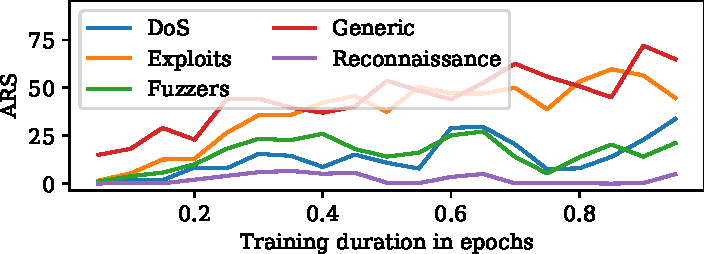
\includegraphics[width=0.98\columnwidth]{./plots/ars/ars_15.pdf}
\caption{\gls{ars} during adversarial training for UNSW-NB15.}
\label{fig:avdistance}
\end{figure}

\renewcommand*{\bibfont}{\small}
\bibliographystyle{ieeetr}
\bibliography{bibliography}


\end{document}
\endinput
%%
%% End of file `sample-sigconf.tex'.
